
%(BEGIN_QUESTION)
% Copyright 2007, Tony R. Kuphaldt, released under the Creative Commons Attribution License (v 1.0)
% This means you may do almost anything with this work of mine, so long as you give me proper credit

Qualitatively graph the response of a controller having {\it both proportional and integral} modes over time to the following changes in process variable, marking the features of the output plot corresponding to proportional action (P) and to integral action (I).

$$\includegraphics[width=15.5cm]{i01595x01.eps}$$

Assume {\it reverse} control action.

\vskip 20pt \vbox{\hrule \hbox{\strut \vrule{} {\bf Suggestions for Socratic discussion} \vrule} \hrule}

\begin{itemize}
\item{} A useful problem-solving strategy is to sketch the P and I actions separately (with their own trends) before combining them to make one final output trend.  A subsection in the {\it Lessons In Industrial Instrumentation} textbook entitled ``Note to Students Regarding Quantitative Graphing'' illustrates this problem-solving technique.
\item{} Why should any controller combine proportional and integral actions?  What is wrong with just using one or the other action alone?
\end{itemize}

\underbar{file i01595}
%(END_QUESTION)





%(BEGIN_ANSWER)

The controller output graph shown here is {\it qualitative} only.  Although drawn to scale (i.e. all changes in the output are properly scaled relative to each other), the scale itself is arbitrary and therefore may not match the scale of your sketch:

$$\includegraphics[width=15.5cm]{i01595x02.eps}$$

%(END_ANSWER)





%(BEGIN_NOTES)

{\bf Proportional control action is where the amount of error tells the output how \underbar{far} to go.}

\vskip 10pt

{\bf Integral control action is where the amount of error tells the output how \underbar{fast} to go.}

\vskip 10pt

{\bf Derivative control action is where \underbar{speed} of the error tells the output how \underbar{far} to go.}

%INDEX% Control, proportional + integral: graphing controller response

%(END_NOTES)


